\documentclass[10pt,a4paper]{article}
\usepackage[a4paper,margin=16mm,top=14mm,bottom=16mm]{geometry}
\usepackage{fontspec}
\setmainfont{Liberation Sans}
\newfontfamily\headingfont{Liberation Serif}
\usepackage{xcolor}
\definecolor{Navy}{HTML}{0B1F33}
\definecolor{NavyTwo}{HTML}{102B47}
\definecolor{GoldAccent}{HTML}{C98C43}
\definecolor{WarmPaper}{HTML}{F7F4EE}
\definecolor{BodyGrey}{HTML}{445565}
\definecolor{RuleGrey}{HTML}{D9E0E6}
\usepackage{hyperref}
\hypersetup{colorlinks=true,urlcolor=Navy,linkcolor=Navy,pdfauthor={Raffaele Mineo},pdftitle={Raffaele Mineo - Academic Curriculum Vitae}}
\usepackage{enumitem}
\usepackage{tabularx}
\usepackage{array}
\usepackage{titlesec}
\usepackage{microtype}
\usepackage{fancyhdr}
\usepackage{lastpage}
\usepackage{parskip}
\usepackage{ragged2e}
\usepackage{graphicx}
\pagestyle{fancy}
\fancyhf{}
\fancyfoot[L]{\scriptsize\color{BodyGrey}Raffaele Mineo — Academic Curriculum Vitae}
\fancyfoot[R]{\scriptsize\color{BodyGrey}\thepage/\pageref{LastPage}}
\renewcommand{\headrulewidth}{0pt}
\renewcommand{\footrulewidth}{0pt}

\setlength{\parindent}{0pt}
\setlength{\parskip}{4pt}
\setlist[itemize]{leftmargin=4.5mm,itemsep=2.2pt,topsep=3pt,parsep=0pt}
\newcommand{\sectionrule}{\vspace{-2pt}\textcolor{GoldAccent}{\rule{16mm}{1.5pt}}\vspace{2pt}}
\titleformat{\section}{\headingfont\color{Navy}\fontsize{15}{18}\selectfont\bfseries}{}{0pt}{}[\vspace{-5pt}\sectionrule]
\titlespacing*{\section}{0pt}{10pt}{5pt}
\titleformat{\subsection}{\color{Navy}\fontsize{10.7}{13}\selectfont\bfseries}{}{0pt}{}
\titlespacing*{\subsection}{0pt}{6pt}{2pt}

\newcommand{\cvrole}[4]{%
\begin{tabularx}{\linewidth}{@{}>{\raggedright\arraybackslash}p{26mm}X@{}}
\textcolor{GoldAccent}{\textbf{#1}} &
\textbf{\color{Navy}#2}\\[-1pt]
& \textit{#3}\\[-1pt]
& \color{BodyGrey}#4
\end{tabularx}\vspace{3pt}}

\newcommand{\cvpub}[4]{%
\begin{tabularx}{\linewidth}{@{}>{\raggedright\arraybackslash}p{11mm}X@{}}
\textcolor{GoldAccent}{\textbf{#1}} &
\textbf{#2}\\[-1pt]
& \small #3\\[-1pt]
& \small\textit{#4}
\end{tabularx}\vspace{3.2pt}}

\begin{document}
\thispagestyle{fancy}

\noindent
\begin{minipage}[t]{0.78\linewidth}
\vspace{0pt}
{\headingfont\fontsize{30}{32}\selectfont\bfseries\color{Navy} Raffaele Mineo}\\[2pt]
{\large\color{NavyTwo}\textbf{Postdoctoral Researcher in Artificial Intelligence}}\\[3pt]
{\small Department of Electrical, Electronic and Computer Engineering (DIEEI), University of Catania}\\[1pt]
{\small Catania, Italy}\\[3pt]
{\fontsize{7.6}{9}\selectfont
\href{mailto:raffaele.mineo@phd.unict.it}{raffaele.mineo[at]phd.unict.it} \quad|\quad
\href{https://scholar.google.com/citations?user=nYSplWUAAAAJ}{Google Scholar} \quad|\quad
\href{https://orcid.org/0000-0002-1171-5672}{ORCID} \quad|\quad
\href{https://www.scopus.com/authid/detail.uri?authorId=58251673400}{Scopus} \quad|\quad
\href{https://www.webofscience.com/wos/author/record/JBJ-0289-2023}{Web of Science}}\\[1pt]
{\fontsize{7.25}{8.6}\selectfont
\href{https://www.semanticscholar.org/author/Raffaele-Mineo/2216463047}{Semantic Scholar} \quad|\quad
\href{https://dblp.org/pid/345/1928.html}{DBLP} \quad|\quad
\href{https://openreview.net/profile?id=~Raffaele_Mineo1}{OpenReview} \quad|\quad
\href{https://github.com/IngRaffaeleMineo}{GitHub} \quad|\quad
\href{http://www.perceivelab.com/team/raffaele-mineo}{PeRCeiVe.AI} \quad|\quad
\href{https://www.researchgate.net/profile/Raffaele-Mineo}{ResearchGate} \quad|\quad
\href{https://it.linkedin.com/in/raffaelemineo}{LinkedIn} \quad|\quad
\href{https://unict.academia.edu/RaffaeleMineo}{Academia.edu}}\\[1pt]
{\scriptsize\color{BodyGrey}Last updated: 15 September 2026}
\end{minipage}\hfill
\begin{minipage}[t]{0.18\linewidth}
\vspace{0pt}
\raggedleft
\fcolorbox{GoldAccent}{white}{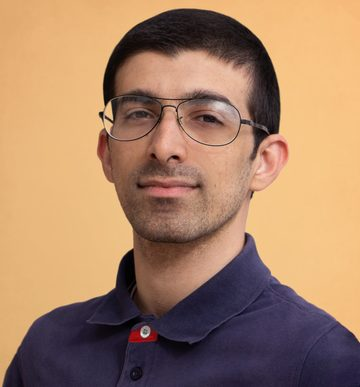
\includegraphics[width=29mm,height=33mm,keepaspectratio]{../assets/raffaele-mineo.jpg}}
\end{minipage}\\[3pt]
\textcolor{GoldAccent}{\rule{\linewidth}{2pt}}

\section{Profile}
\color{BodyGrey}
I develop artificial intelligence methods that connect perception with clinically and operationally meaningful information. My research spans cardiovascular imaging and virtual physiology, multimodal and radar-based sign language understanding, continual and federated learning, vision-language adaptation, and efficient AI for resource-constrained hardware. The common thread is the design of models that remain useful under realistic acquisition, privacy, data and compute constraints, with attention to translational and deployable outcomes.
\color{black}

\section{Academic positions and research experience}
\cvrole{2024--present}{Postdoctoral Researcher / Research Fellow}{University of Catania — DIEEI}{HORIZON Europe NEUROKIT2E: knowledge distillation and meta-learning for on-chip AI inference; medical imaging, multimodal learning, efficient/embedded AI and project research activities.}
\cvrole{2019--present}{Research member / assistant}{PeRCeiVe.AI Lab, University of Catania}{Computer vision, pattern recognition, medical imaging, multimodal AI and applied deep learning.}
\cvrole{2023--present}{AI consulting and industrial R\&D collaboration}{DeepSensing S.r.l., Catania}{Deep-learning systems for industrial inspection; multi-GPU experimentation; edge and neuromorphic computing; predictive reliability; Horizon-project activities and KPI-oriented validation.}
\cvrole{from 2023}{Research collaboration}{STMicroelectronics R\&D Power and Discrete, Catania}{Artificial intelligence for modeling and predictive reliability in automotive and power-electronics contexts.}

\section{Education}
\cvrole{completed 2026}{National PhD in Artificial Intelligence — Health and Life Sciences}{University Campus Bio-Medico of Rome, with University of Catania affiliation}{37th cycle.}
\cvrole{2019--2021}{M.Sc. in Computer Engineering}{University of Catania}{110/110 cum laude. Thesis: \textit{Prediction of paroxysmal events through an anomaly detection approach based on Transformers}.}
\cvrole{2016--2019}{B.Sc. in Computer Engineering}{University of Catania}{99/110. Thesis on the design and implementation of an optical data-communication interface for Li-Fi applications.}
\cvrole{2016}{Scientific High School Diploma}{Liceo Scientifico “L. Da Vinci”, Floridia}{97/100.}

\section{Research themes}
\begin{itemize}
\item \textbf{Cardiovascular AI and virtual physiology:} coronary angiography, FFR/iFR estimation, spatio-temporal modeling, clinically meaningful representations and translational validation.
\item \textbf{Multimodal and privacy-aware sensing:} radar, RGB, depth, skeleton and multimodal learning for sign language recognition and accessible healthcare communication.
\item \textbf{Adaptive and distributed learning:} personalized continual/incremental learning, self-supervision, federated learning and prompt-based adaptation.
\item \textbf{Efficient and embedded AI:} knowledge distillation, post-training quantization, edge inference, STM32/embedded deployment and resource-constrained optimization.
\item \textbf{Applied machine intelligence:} cognitive assessment, industrial inspection, predictive reliability, anomaly detection, volcanology and data-driven engineering systems.
\end{itemize}

\section{Patents, inventions and technology transfer}
\cvrole{2026}{Angiographic image processing method and system}{Italian patent no. 102024000014434; PCT/IB2025/056252; WO 2025/262634 A1}{Italian patent granted by UIBM on 20 July 2026. The patent family protects AI-based angiographic processing underpinning the STARFLOW line of research.}
\cvrole{pending}{Biometric safety system and method for estimating a user hazard condition and triggering an emergency stop}{Italian patent application — under review}{Inventors include Raffaele Mineo, Paolo Soda, Simone Palazzo and Concetto Spampinato.}
\cvrole{in development}{AI Framework for Automotive Microcontrollers}{Patent filing / invention under development}{Inventors include Francesco Rundo, Raffaele Mineo, Simone Palazzo and Concetto Spampinato.}

\section{Academic service and leadership}
\subsection{Editorial roles}
\begin{itemize}
\item Associate Editor — Frontiers in Communication (2026–)
\item Lead Guest Editor — Cognitive Computation, Special Issue “Cognitive and Multimodal Sign Language Processing: Recognition, Understanding, Translation, Generation, and Inclusive Interaction” (2026)
\end{itemize}
\subsection{Area-chair, program and organizing roles}
\begin{itemize}
\item Area Chair — MICCAI 2026
\item Area Chair — IJCNN 2027
\item Organizing Committee — IEEE ISBI 2026, Associate to Technical Program Chairs
\item Paper Selection Committee — IPMI 2027
\item Lead Post-Day Workshops \& Challenges Chair — MIDL 2027
\end{itemize}
\subsection{Workshops, challenges and special sessions}
\begin{itemize}
\item Lead Organizer — IEEE ISBI 2026 Special Session: “Privacy-Aware, Data-Efficient AI via Personalized Incremental and Federated Learning in Healthcare”
\item Workshop Chair — ICCV 2025: 1st International Workshop on Multimodal Sign Language Recognition + 1st SignEval Challenge
\item Workshop Chair — ACM Multimedia 2025: 2nd International Workshop on Personalized Incremental Learning in Medicine
\item Workshop Chair — CVPR 2026: 2nd International Workshop on Multimodal Sign Language Recognition + 2nd SignEval Challenge
\end{itemize}
\subsection{Journal reviewing}
\begin{itemize}
\item IEEE Transactions on Medical Imaging (TMI), since 2025
\item IEEE Open Journal of the Computer Society (OJCS), since 2025
\item Computer Vision and Image Understanding (CVIU), since 2023
\item Machine Vision and Applications (MVAP), since 2023
\item ACM Transactions on Intelligent Systems and Technology (TIST), since 2024
\item Nature Communications, since 2025
\item BioData Mining, since 2026
\item Disability and Rehabilitation: Assistive Technology, since 2026
\item Frontiers in Digital Health, since 2026
\item IJCCE, since 2026
\item JIIM, since 2026
\item IEEE Transactions on Biomedical Engineering (TBME), since 2026
\end{itemize}
\subsection{Conference and workshop reviewing}
\begin{itemize}
\item \textbf{Conferences:} ECCV 2024; BIBM 2024; RTSI 2024; ISBI 2026; MICCAI 2026; IJCNN 2026; EMBC 2026; NeurIPS 2026; AAAI 2027.
\item \textbf{Workshops:} MICCAI AIPAD 2024; IJCNN SPAN 2025; CVPR MSLR 2026; ICPR CVBMC 2026; MICCAI AFRICAI 2026.
\end{itemize}
\subsection{Volunteering, mentoring and research advising}
\begin{itemize}
\item Mentor — GreenMindAI Catania Hackathon 2025
\item Student Volunteer — ACM Multimedia 2025
\item Proctor — IEEEXtreme 20.0 (2026)
\item Research Advisor — RISE-MICCAI 2027 Publication Accelerator
\end{itemize}

\section{Peer-reviewed journal articles}
\cvpub{2024}{Non-invasive physiological assessment of intermediate coronary stenoses from plain angiography through artificial intelligence: the STARFLOW system \textcolor{GoldAccent}{\textsuperscript{*}}}{Ovidio De Filippo*, \textbf{Raffaele Mineo}*, Michele Millesimo, Wojciech Wańha, Federica Proietto Salanitri, Antonio Greco, Antonio Maria Leone, Luca Franchin, Simone Palazzo, Giorgio Quadri, Domenico Tuttolomondo, Enrico Fabris, Gianluca Campo, Alessandra Truffa Giachet, Francesco Bruno, Mario Iannaccone, Giacomo Boccuzzi, Nicola Gaibazzi, Ferdinando Varbella, Wojciech Wojakowski, Michele Maremmani, Guglielmo Gallone, Gianfranco Sinagra, Davide Capodanno, Giuseppe Musumeci, Paolo Boretto, Pawel Pawlus, Andrea Saglietto, Francesco Burzotta, Marco Aldinucci, Daniela Giordano, Gaetano Maria De Ferrari, Concetto Spampinato, Fabrizio D'Ascenzo}{European Heart Journal-Quality of Care and Clinical Outcomes}
\cvpub{2024}{A Convolutional-Transformer Model for FFR and iFR Assessment From Coronary Angiography}{\textbf{Raffaele Mineo}, F Proietto Salanitri, G Bellitto, I Kavasidis, O De Filippo, M Millesimo, GM De Ferrari, M Aldinucci, D Giordano, S Palazzo, F D’Ascenzo, C Spampinato}{IEEE Transactions on Medical Imaging}

\section{Conference and workshop publications}
\cvpub{2026}{SignEval 2026 Challenges Results \textcolor{GoldAccent}{\textsuperscript{*}}}{Ahmed Abul Hasanaath, \textbf{Raffaele Mineo}, Hamzah Luqman, Sarah Alyami, Maad Alowaifeer, Amelia Sorrenti, Gaia Caligiore, Sabina Fontana, Egidio Ragonese, Giovanni Bellitto, Federica Proietto Salanitri, Concetto Spampinato, Motaz Alfarraj, Mufti Mahmud, Simone Palazzo, Nour Imane Zeghib}{IEEE/CVF Conference on Computer Vision and Pattern Recognition Workshops}
\cvpub{2026}{Advancing Healthcare with Multimodal AI: Enhanced Diagnosis, Cognitive Monitoring, and Inclusive Medical Communication}{\textbf{Raffaele Mineo}}{International Conference on Medical Image Computing and Computer-Assisted Intervention}
\cvpub{2026}{A Benchmark for Radar-Based Italian Sign Language Recognition using Frequency-Domain Range-Time Maps}{\textbf{Raffaele Mineo}, Amelia Sorrenti, Gaia Caligiore, Federica Proietto Salanitri, Giovanni Bellitto, Senya Polikovsky, Sabina Fontana, Egidio Ragonese, Concetto Spampinato, Simone Palazzo}{IEEE/CVF Conference on Computer Vision and Pattern Recognition Workshops}
\cvpub{2025}{Timely Predicting Power Mosfet Failure in EV: AI Based Metodology and Deployment at the Edge}{Robin Faro, Francesco Cancelliere, Alesssandro Strano, \textbf{Raffaele Mineo}}{2025 IEEE Symposia on Computational Intelligence for Energy, Transport and Environmental Sustainability (CIETES Companion)}
\cvpub{2025}{The SignEval 2025 Challenge at the ICCV Multimodal Sign Language Recognition Workshop: Results and Discussion \textcolor{GoldAccent}{\textsuperscript{*}}}{Hamzah Luqman*, \textbf{Raffaele Mineo}*, Murtadha Aljubran, Ahmed Abul Hasanaath, Amelia Sorrenti, Sarah Alyami, Sadam Al-Azani, Maad Alowaifeer, JiHwan Moon, Vaclav Javorek, Tomas Zelezny, Marek Hruz, Gaia Caligiore, Silvio Giancola, Senya Polikovsky, Motaz Alfarraj, Sabina Fontana, Mufti Mahmud, Muhammad Haris Khan, Kamrul Islam, Sevgi Gurbuz, Egidio Ragonese, Giovanni Bellitto, Federica Proietto Salanitri, Concetto Spampinato, Simone Palazzo}{Proceedings of the IEEE/CVF International Conference on Computer Vision}
\cvpub{2025}{Text-Aligned Radar-Based Sign Language Recognition for Healthcare Communication}{\textbf{Raffaele Mineo}, Amelia Sorrenti, Gaia Caligiore, Federica Proietto Salanitri, Giovanni Bellitto, Senya Polikovsky, Sabina Fontana, Egidio Ragonese, Concetto Spampinato, Simone Palazzo}{Proceedings of the IEEE/CVF International Conference on Computer Vision}
\cvpub{2025}{Radar-Based Imaging for Sign Language Recognition in Medical Communication}{\textbf{Raffaele Mineo}, Gaia Caligiore, Federica Proietto Salanitri, Isaak Kavasidis, Senya Polikovsky, Sabina Fontana, Egidio Ragonese, Concetto Spampinato, Simone Palazzo}{International Conference on Medical Image Computing and Computer-Assisted Intervention}
\cvpub{2025}{PCB-SAID: A Low-Cost Camera-Based Dataset for Few-Shot SMD Assembly Inspection}{\textbf{Raffaele Mineo}, Amelia Sorrenti, Robin Faro, Gabriele Mineo, Francesco Cancelliere, Alberto Faro}{Proceedings of the IEEE/CVF International Conference on Computer Vision}
\cvpub{2025}{Memory-Augmented Prompt Tuning for Self-Supervised Continual Learning in Medical Imaging}{-}{International Workshop on Personalized Incremental Learning in Medicine (PILM)}
\cvpub{2025}{Learning Joint Text and Visual Tokens in CLIP for Medical Image Analysis}{\textbf{Raffaele Mineo}, Giovanni Bellitto, Federica Proietto Salanitri, Rutger Hendrix, Concetto Spampinato, Simone Palazzo}{Proceedings of the 2nd International Workshop on Multimedia Computing for Health and Medicine}
\cvpub{2025}{HC-PTQ: Poincaré-Based Hyperbolic Clustering for Data-Free Quantization of Vision Transformers}{\textbf{Raffaele Mineo}, Simone Palazzo, Concetto Spampinato, Francesco Rundo}{Proceedings of the IEEE/CVF International Conference on Computer Vision}
\cvpub{2025}{Conditional Visuo-Textual Prompt Learning for Medical Image Analysis}{\textbf{Raffaele Mineo}, Giovanni Bellitto, Federica Proietto Salanitri, Rutger Hendrix, Ulas Bagci, Daniela Giordano, Concetto Spampinato, Simone Palazzo}{2025 IEEE 22nd International Symposium on Biomedical Imaging (ISBI)}
\cvpub{2025}{Automated MoCA Score Estimation Using Eye-Gaze Data and Vision Transformers}{\textbf{Raffaele Mineo}, Isaak Kavasidis, Federica Proietto Salanitri, Lisa Passarello, Giovanni Piccininno, Vincenzo Masciale, Alessandro Anselmo, Cristiano Convertino, Domenico Rotondi, Nicola Laurieri, Simone Palazzo, Concetto Spampinato, Manuela Pennisi, Daniela Giordano}{2025 IEEE 38th International Symposium on Computer-Based Medical Systems (CBMS)}
\cvpub{2024}{Sign Language Recognition for Patient-Doctor Communication: A Multimedia/Multimodal Dataset}{\textbf{Raffaele Mineo}, Gaia Caligiore, Concetto Spampinato, Sabina Fontana, Simone Palazzo, Egidio Ragonese}{2024 IEEE 8th Forum on Research and Technologies for Society and Industry Innovation (RTSI)}
\cvpub{2024}{Multisource Approaches to Italian Sign Language (LIS) Recognition: Insights from the MultiMedaLIS Dataset \textcolor{GoldAccent}{\textsuperscript{*}}}{Gaia Caligiore*, \textbf{Raffaele Mineo}*, Concetto Spampinato, Egidio Ragonese, Simone Palazzo, Sabina Fontana}{2024 10th Italian Conference on Computational Linguistics (CLiC-it)}
\cvpub{2024}{Magnifying facial micro-movements for cognitive evaluation}{\textbf{Raffaele Mineo}, Federica Proietto Salanitri, Lisa Passarello, Alberto Sardella, Laura Messina, Manuela Pennisi, Daniela Giordano, Simone Palazzo, Concetto Spampinato}{2024 46th Annual International Conference of the IEEE Engineering in Medicine and Biology Society (EMBC)}
\cvpub{2024}{Coronary Artery Stenosis Assessment in X-Ray Angiography Through Spatio-Temporal Attention for Non-Invasive FFR and iFR Estimation}{\textbf{Raffaele Mineo}, Federica Proietto Salanitri, Giovanni Bellitto, Ovidio De Filippo, Fabrizio D'Ascenzo, Simone Palazzo, Concetto Spampinato}{Proceedings of the 17th International Joint Conference on Biomedical Engineering Systems and Technologies - Volume 1: BIOIMAGING}
\cvpub{2023}{FeDETR: A Federated Approach for Stenosis Detection in Coronary Angiography}{\textbf{Raffaele Mineo}, Amelia Sorrenti, Federica Proietto Salanitri}{International Conference on Image Analysis and Processing}
\cvpub{2023}{Ensemble and personalized transformer models for subject identification and relapse detection in e-prevention challenge}{Salvatore Calcagno, \textbf{Raffaele Mineo}, Daniela Giordano, Concetto Spampinato}{ICASSP 2023-2023 IEEE International Conference on Acoustics, Speech and Signal Processing (ICASSP)}
\cvpub{2023}{Dynamic Graph Attention: Unraveling Spatio-Temporal Synchrony in EEG Data}{Federica Proietto Salanitri, Giovanni Bellitto, \textbf{Raffaele Mineo}, Matteo Pennisi, Amelia Sorrenti, Salvatore Calcagno, Daniela Giordano, Simone Palazzo, Concetto Spampinato}{2023 IEEE International Conference on Bioinformatics and Biomedicine (BIBM)}
\cvpub{2023}{BioTrak: A Blockchain-based Platform for Food Chain Logistics Traceability}{Alessia Spitalleri, Isaak Kavasidis, Vincenzo Cartelli, \textbf{Raffaele Mineo}, Francesco Rundo, Simone Palazzo, Concetto Spampinato, Daniela Giordano}{2023 International Conference on Intelligent Computing, Communication, Networking and Services (ICCNS)}
{\small\textcolor{BodyGrey}{\textsuperscript{*} Joint first author where explicitly indicated in the supplied publication list.}}

\section{Other scholarly and research outputs}
\cvpub{2025}{Proceedings of the International Workshop on Personalized Incremental Learning in Medicine (PILM ’25)}{Simone Palazzo, Giovanni Bellitto, \textbf{Raffaele Mineo}, Amelia Sorrenti, Camila Gonzalez, Angelo Porrello, Lorenzo Bonicelli}{ACM Multimedia 2025}
\cvpub{2021}{VOLcano UNrest Detection (VolUnD) Toolkit}{\textbf{R. Mineo}, P. Spadaro, F. Cannavò, S. Palazzo, A. Cannata, C. Spampinato}{Zenodo}
\cvpub{2021}{EUROVOLC - Deliverable Report - D9.3 Machine learning tool kit and database}{S. Palazzo, \textbf{R. Mineo}, C. Spampinato, F. Cannavò, A. Cannata, C. Montagna, J. M. Saurel, O. Geber, A. Lemarchand}{HORIZON 2020 EUROVOLC Project}
\subsection{Current / additional scholarly outputs represented in the supplied metadata}
\cvpub{n.d.}{Personalized Incremental Learning in Medicine: A Comprehensive Survey of Methods, Challenges, and Future Directions}{-}{Manuscript / scholarly output}
\cvpub{n.d.}{Anomaly Detection in Volcanic Seismic Data Using Deep Learning: A Case Study on Mt. Etna}{-}{IEEE Access — metadata entry; status/year to update}

\section{Research projects and collaborations}
\begin{itemize}
\item \textbf{HORIZON Europe — NEUROKIT2E} (Grant Agreement 101112268): research on knowledge distillation and meta-learning for on-chip AI inference; contributions also spanning embedded/edge AI and performance evaluation.
\item \textbf{HORIZON Europe — EdgeAI related activities:} deep-learning algorithms for defect detection on electronic boards and wood products; multi-GPU and edge-computing experimentation; neuromorphic approaches; KPI and functional/non-functional requirement evaluation.
\item \textbf{HORIZON 2020 — EUROVOLC} (Grant Agreement 731070): machine-learning toolkit and database for volcanic-unrest analysis; VolUnD toolkit and D9.3 deliverable.
\item Research collaborations with the \textbf{Istituto Nazionale di Geofisica e Vulcanologia (INGV), Catania}; \textbf{AOU Città della Salute e della Scienza, Turin}; \textbf{Max Planck Institute for Intelligent Systems, Tübingen}; and \textbf{STMicroelectronics R\&D Power and Discrete, Catania}.
\item Industrial R\&D / consulting collaboration with \textbf{DeepSensing S.r.l., Catania}.
\end{itemize}

\section{Teaching}
\begin{itemize}
\item Teaching Tutor, \textbf{Database and Web Programming}, Computer Engineering, University of Catania — multiple editions, 2022--2025.
\item Teaching Tutor, \textbf{Fundamentals of Computer Science}, Industrial Engineering, University of Catania — 2022--2023.
\end{itemize}

\section{Professional memberships and technical communities}
\begin{itemize}
\item CVPL / PeRCeiVe research community (since 2019)
\item IEEE Engineering in Medicine and Biology Society (EMBS), since 2024
\item IEEE Signal Processing Society (SPS), since 2025
\item Association for Computing Machinery (ACM), since 2025
\item ACM SIGMM, since 2025
\item IEEE PAMI Technical Community, since 2026
\item IEEE Bio Imaging and Image Processing (BIIP) Technical Committee, since 2026
\end{itemize}

\section{Technical competencies}
\begin{itemize}
\item \textbf{Artificial intelligence and data:} AI for Medicine, machine learning, deep learning, data acquisition systems, PyTorch, Keras, TensorFlow, R, SQL, MySQL, PostgreSQL.
\item \textbf{Programming:} Python, C, C++, C\#, Java, JavaScript, TypeScript, Go, PHP, AutoIt, OpenGL, QML, Qt Framework / Qt Quick, ASP.NET, Angular, Laravel, Node.js.
\item \textbf{Embedded systems and sensing:} STM32 firmware, Arduino, Infineon Radar SDK, Intel RealSense SDK, Microsoft Kinect SDK, Stereolabs ZED SDK, edge computing, multi-GPU systems.
\item \textbf{Engineering and development tools:} Android Studio, Atollic TrueSTUDIO, Eclipse, IntelliJ IDEA, Qt Creator, Visual Studio, Visual Studio Code, AutoCAD, Autodesk EAGLE, Autodesk Tinkercad.
\item \textbf{Web, systems and networks:} HTML, CSS, SCSS, JSON, client/server applications, network architecture, operating systems.
\item \textbf{Media, graphics and productivity:} Adobe Illustrator, Photoshop, Acrobat, After Effects, Premiere Pro, Blender, CorelDRAW, Unity, Microsoft Office, Excel and PowerPoint.
\end{itemize}

\section{Languages}
\begin{itemize}
\item Italian — native
\item English — B1 (Cambridge certified)
\item French — A1
\item Spanish — A1
\end{itemize}

\section{Professional qualifications, certifications and training}
\begin{itemize}
\item Italian State Examination and professional qualification as Information Engineer (2021)
\item Mensa Italia certificate / membership credential
\item ECDL Core AICA (2014)
\item Cambridge English B1 Preliminary (2014); Cambridge English A2 Key (2012)
\item Würth Elektronik Italia — Power Expert technical training (2021)
\item Coursera / DeepLearning.AI: Neural Networks and Deep Learning; Improving Deep Neural Networks; Structuring Machine Learning Projects; Convolutional Neural Networks; Sequence Models; Deep Learning Specialization
\item Coursera: AI for Medical Diagnosis; AI for Medical Prognosis; AI for Medical Treatment; AI for Medicine Specialization; Detecting COVID-19 with Chest X-Ray using PyTorch
\item Coursera / DeepLearning.AI: Build Basic GANs; Build Better GANs; Apply GANs; Generative Adversarial Networks Specialization
\end{itemize}

\section{Additional hands-on technical background}
\color{BodyGrey}
Electronic-board repair for household appliances; desktop/laptop/smartphone/tablet hardware and software repair; installation and maintenance experience with television systems, alarm systems, video surveillance, structured cabling and selected plumbing/HVAC systems; electro-welding and carpentry; preparation of technical-estimative reports and IT appraisals.
\color{black}

\end{document}
